\begin{mainquestion}{sourcefollower}{Source Follower Measurement}

\begin{center}
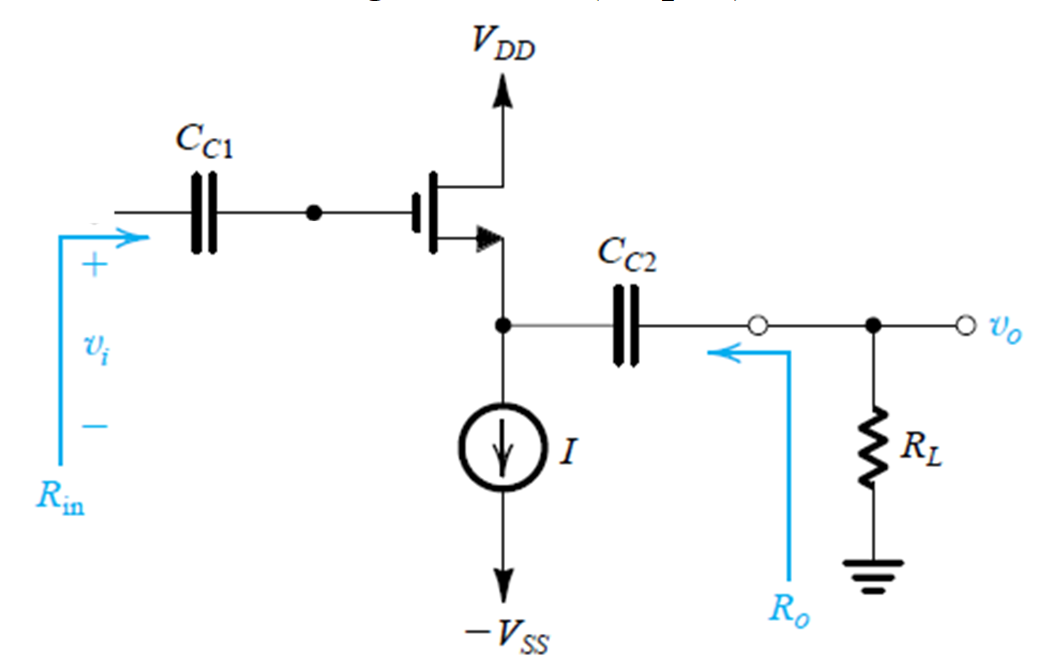
\includegraphics[width=4.5in]{image7.png}
\end{center}

A source-follower circuit is shown below. With $\mathbf{R}_{\mathbf{L}}$ removed, the open-circuit voltage gain $\mathbf{A}_{\mathbf{vo}} = \frac{\mathbf{v}_{\mathbf{o}}}{\mathbf{v}_{\mathbf{i}}}$ is carefully measured and found to be 0.95. Then, when $\mathbf{R}_{\mathbf{L}}$ is connected and its value is varied, we find the gain is halved at $\mathbf{R}_{\mathbf{L}} = 850\ \Omega$. If the amplifier remained linear during the measurement, what are the values of $\mathbf{g}_{\mathbf{m}}$ and $\mathbf{r}_{\mathbf{o}}$?

\begin{partquestion}{gm}{Find $\mathbf{g}_{\mathbf{m}}$}
\begin{answer}
The open-circuit gain of the source follower (common-drain) stage without a load is:

\[
A_{vo} = \frac{v_{o}}{v_{i}} = \frac{g_{m} r_{o}}{1 + g_{m} r_{o}} = 0.95.
\]

With a load, the total gain is a voltage divider:

\[
A_{v} = A_{vo} \frac{R_{L}}{R_{L} + R_{o}}.
\]

If this gain is halved by connecting $R_{L} = 850\ \Omega$, then $R_{o} = 850\ \Omega$.

Since $R_{o} = \frac{r_{o}}{1 + g_{m} r_{o}}$, taking the ratio of the first and third equations gives:

\[
g_{m} = \frac{A_{vo}}{R_{o}} = \frac{0.95}{850} = 1.118\ \text{mS}.
\]
\end{answer}
\end{partquestion}

\begin{partquestion}{ro}{Find $\mathbf{r}_{\mathbf{o}}$}
\begin{answer}
Use the relationship between $R_{o}$, $g_{m}$, and $r_{o}$:

\[
R_{o} = \frac{r_{o}}{1 + g_{m} r_{o}} = 850\ \Omega.
\]

Solve for $r_{o}$ using the measured values:

\begin{align*}
    r_o &= \frac{R_o}{1 - R_o g_m} \\
    &= \frac{850}{1 - 850(0.001118)} = \qty{17}{\kilo\ohm}
\end{align*}

\end{answer}
\end{partquestion}

\end{mainquestion}
